\section{Issues Encountered So Far}

\subsection*{Non-Deterministic Nature of the Extraction Algorithm}

The extraction algorithm used by RA is non-deterministic,
meaning that for the same input code, the output of the extraction process can
vary. This results in different versions of semantically equivalent but
syntactically distinct code. In other words, while the extracted code maintains
the same functionality, its structure and readability can change between runs.
This poses a significant challenge for testing the tool, as each run may yield
different outputs for the same input, making consistent verification difficult. \\
For example in Figure \ref{fig:issue1}, a test of function extraction, RA may choose to pass
variables by reference to the extracted function, dereferencing them inside the
function body. In another instance, it might pass the same variables by
ownership, altering the code's appearance but not its behavior. While both
versions of the code will likely compile to identical machine code, the
readability and clarity of the resulting code can vary.

\begin{figure}[H]
    \centering
    \sbox\mysavebox{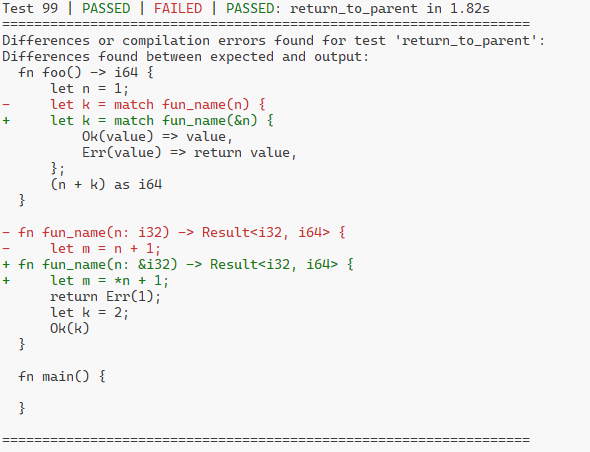
\includegraphics[width=0.9\columnwidth]{Figures/issue_1.png}}
    \usebox\mysavebox
    \par
    \begin{minipage}{\wd\mysavebox}
        \caption{An example of the non-deterministic nature of the extraction
        algorithm. \textcolor{red}{Red is expected output}, \textcolor{green}{green is the
        returned code} \label{fig:issue1}.}
    \end{minipage}
\end{figure}


\subsection*{Performance Bottlenecks in Large Codebases}

The extraction tool's performance is a notable limitation in its current form.
Since it is designed to be modular and not tied to any specific codebase, it
must build a representation of the entire project to perform code extraction.
While this approach works well for small, isolated test cases, it becomes
inefficient when applied to larger, project-scale codebases. In such cases, the
tool faces significant performance bottlenecks. \\
To address this, the tool will need to either (a) operate on a targeted subset
of the codebase, focusing only on the relevant files and functions, or (b)
efficiently cache and reuse results from RA's existing analysis
to avoid redundant computations. Both approaches present technical challenges
that require careful consideration.